\section{Zadanie interpolacji}
	\begin{frame}{3.1 Zadanie interpolacji}

	\begin{figure}[h]
			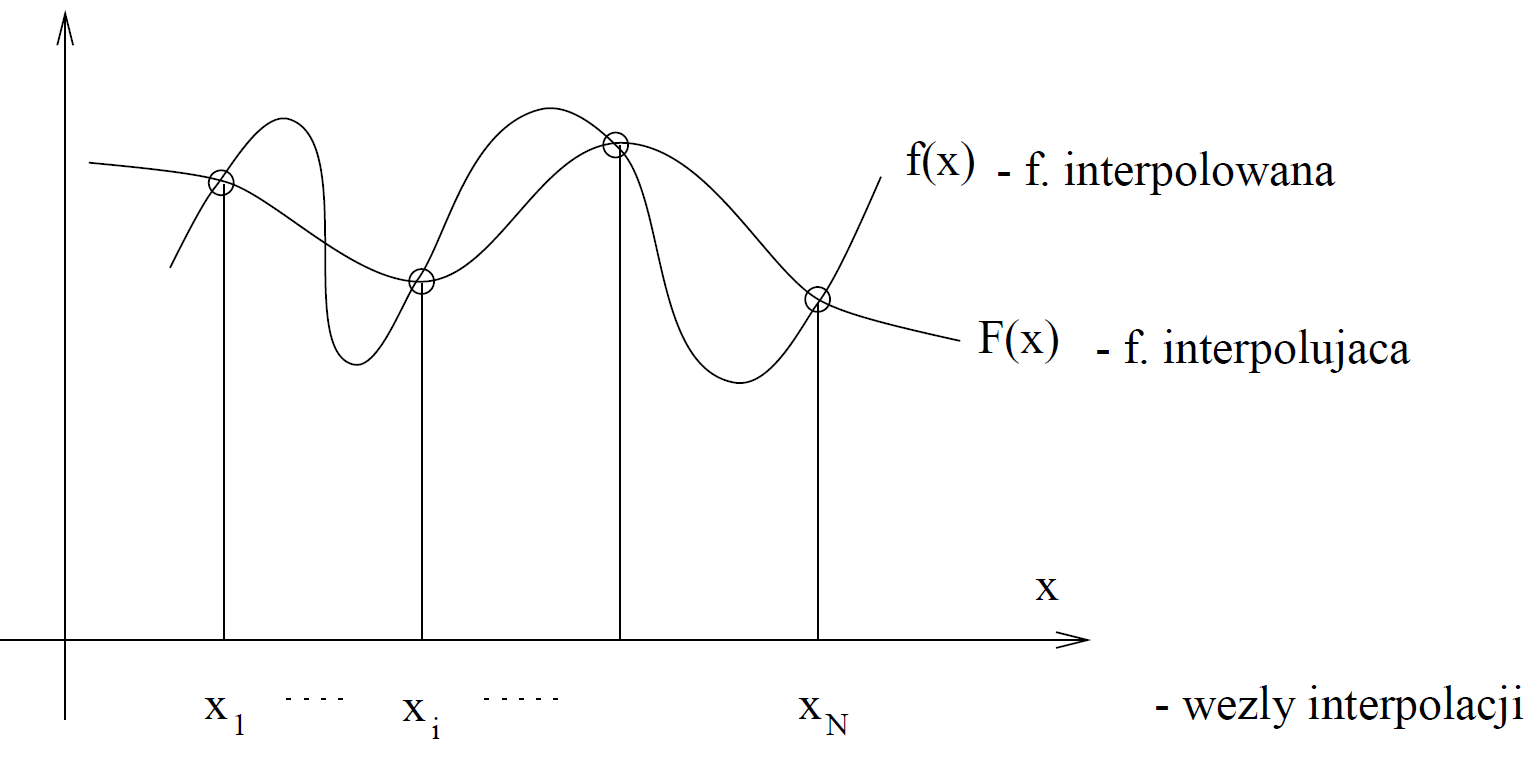
\includegraphics[width=1 \linewidth]{img/3/interpol_3_1}
	\end{figure}
    \end{frame}
    
    \begin{frame}
	\textcolor{blue}{Dane:}

	\begin{itemize}
	\item $[a,\ b]$

	\item $\{(x_{i},\ f_{i}=f(x_{i})),\ i=1,\ 2,\ .\ .\ .\ ,\ N\}$
	$\newline$
    \end{itemize}
	\textcolor{blue}{Szukane:}
	\begin{itemize}
	\item $F(x)$ - funkcja interpolująca $\rightarrow $ wartości w $x \neq x_{i}$ \\
    \item $E(x)$ - oszacowanie błędu interpolacji
    \end{itemize}
    $\newline$
    pod warunkiem: \\
    $F(x_{i}) = f_{i}$ - takie same w węzłach
    $\newline$ \\
    Odmiana:
    poza $f(x_{i})$ dane także $f^{(k)}(x_{i})$
    
	\end{frame}